\chapter{Calibration of the EM calorimeter}
\label{sec:Calibration}

The amount of energy that the EM calorimeter registers differs very much from the total energy of the particle, that needs to be reconstructed. There are several reasons for that: some energy is deposited in the presampler (i.e. outside the calorimeter), some energy is deposited far away from the main cluster and is not registered by the clustering algorithms, but most importantly, lots of energy is deposited in the so-called dead material. The accordeon structure of the central- and the tube structure of the forward- calorimeters both have most of it's mass composed of the non-sensitive materials. Because of these problems, the calorimeters must be calibrated in order to reconstruct the energy of the particles. The process consists of the $\chi^{2}$ minimisation of the theoretically predicted, reconstructed energy and the truth (initial) energy of the MC sample. The MC sample is simulated using Geant4, the deposited energy is calculated based on the precise geometry model of the detector, the energy of the initial particles is then reconstructed using the theoretical model with several free parameters, and the parameters are then locked with the use of the approximation method.

\section{Theoretical overview}

The theretically predicted formula for reconstruction of the energy is as follows

\begin{equation}
\label{eq:calib_theory}
\begin{gathered}
E_{e/\gamma} = \underbrace{a(E^{acc}_{tot}, |\eta|) + b (E^{acc}_{tot}, |\eta|) \cdot E^{clLAr}_{ps} + c (E^{acc}_{tot}, |\eta|) \cdot (E^{clLAr}_{ps})^{2}}_\text{energy in front} \\
+ \underbrace{\frac{s^{Acc}_{cl}(X,\eta)}{f_{out}(X,|\eta|)} \cdot \left( \sum\limits_{i=1,3} E^{clLAr}_{i} \right)}_\text{energy in accordion}
 \cdot \underbrace{(1+f_{leak}(X,|\eta|)) \vphantom{\left( \sum\limits_{i=1,3} E^{clLAr}_{i} \right)}}_\text{longitudal leakage}
 \cdot F(|\eta|,\varphi) \,,
\end{gathered}
\end{equation}
where

\begin{itemize}
\item $a(E^{acc}_{tot}, |\eta|)$, $b (E^{acc}_{tot}, |\eta|)$ and $c (E^{acc}_{tot}, |\eta|)$ are the parameters that are used to correct the reconstructed energy based on the total energy deposited in the accordeon structure ($E^{acc}_{tot}$) and $\eta$. The first two parameters are commonly called offset and slope. The third parameter was assumed to be negligible ($c=0$).
\item $X$ is the longitudinal barycenter of the EM shower, thus representing shower depth. It is calculated as
\begin{equation}
\label{eq:calib_barycenter}
X = \frac{\sum\limits^{3}_{i=0}E^{clLAr}_{i} \cdot X_{i}}{\sum\limits^{3}_{i=0}E^{clLAr}_{i}} \,,
\end{equation}
where $E^{clLAr}_{i}$ is the energy deposited in on of the compartment of the calorimeter: presampler in case $i=0$ and strip, middle and back for the subsequent $i$ values respectively, and $X_{i}$ is the depth, expressed in radiation length, of the longitudinal centre of each compartment computed from the centre of the ATLAS detector. The parameters $E^{clLAr}_{i}$ are also used in eq.~\ref{eq:calib_theory} directly.
\item $E^{clLAr}_{ps}$ is the part of the cluster energy measured in the presampler and corrected for the energy deposited in the passive materials.
\item $s^{Acc}_{cl}(X,\eta)$ is a correction factor to the Accordion sampling fraction in the cluster.
\item $f_{out}(X,|\eta|)$ is the correction for the lateral leakage of the shower, i.e. the energy deposited in the calorimeter outside the cluster.
\item $f_{leak}(X,|\eta|)$ is the correction for the longitudal leakage of the shower.
\item $F(|\eta|,\varphi)$ is the correction for the expected performance of the ATLAS detector, as described in~\cite{lib:ATLAS_perf}.
\end{itemize}

As there is no presampler in the region of the outer wheel of the EMEC, as well as the forward region of the detector (can be effectively summarized as $|\eta|>1.8$), the $E^{clLAr}_{ps}$ parameter is parameterized there as the function of the barycenter (see eq.~\ref{eq:calib_barycenter}) and the fractions of the energy deposited in every compartment of the calorimeter.

The coefficients of this equation were optimised with several MC samples with different fixed energies ranged from 5 GeV to 1 TeV.

The reconstruction of the converted and unconverted photons is done using the same techinque as for the electrons, with the coefficients approximation being done separately.

\section{Calibration procedures}

\begin{figure}
\center{
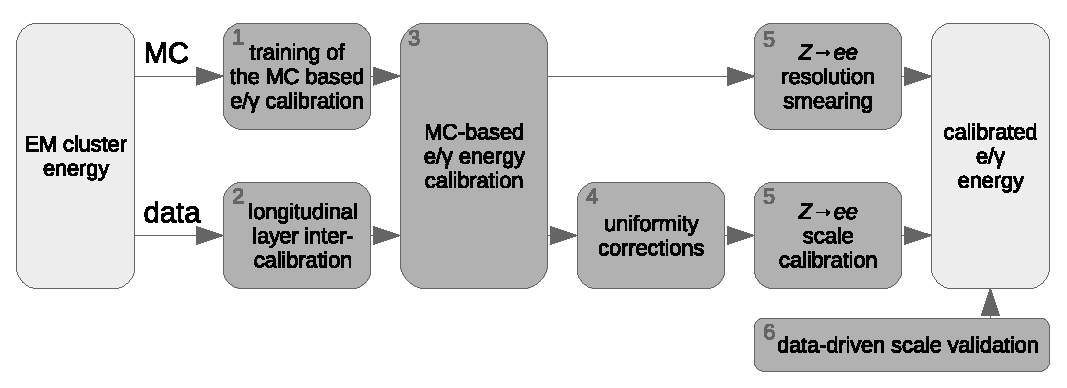
\includegraphics[width=1.0\textwidth]{figures/CALIB_main.eps}
\caption{Schematic overview of the stages of the calibration procedures for the electrons and photons in ATLAS.}
\label{fig:calib}}
\end{figure}

In order to reconstruct the energy of the EM-particles, several procedures are conducted, the overview of which can be seen in Fig.~\ref{fig:calib}. The steps are as follows:

\begin{enumerate}
\item The EM cluster properties, including its longitudinal development, and additional information from the ATLAS inner tracking system, are calibrated to the original electron and photon energy in simulated MC samples. The calibration constants are determined using a multivariate algorithm (MVA), with its optimisation being performed separately for electrons and converted and unconverted photons. For this calibration to work properly, the geometry of the detector must be described as precise as possible, so that the interactions of the particles with the detector material were accurate. The material distribution is measured in data using the ratio of the first-layer energy to the second-layer energy in the longitudinally segmented EM calorimeter. Measuring this ratio in data with different samples (electrons and unconverted
photons) allows a precise determination of the amount of material in front of the calorimeter and provides some sensitivity to its radial distribution.
\item Since the EM calorimeter is longitudinally segmented, the step is taken to equalize the scales of the different longitudinal layers in data with respect to simulation, prior to the determination of the overall energy scale, in order to ensure the correct extrapolation of the response in the full $p_{T}$ range used in the various analyses.
\item The MC-based $e/\gamma$ response calibration is applied to the cluster energies recorded both from collision data and MC simulated samples.
\item A set of corrections are implemented to account for response variations not included in the simulation in specific detector regions, e.g. non-optimal high-voltage regions, geometric effects such as the intermodule widening or biases associated with the LAr calorimeter electronic calibration.
\item The overall electron response in data is calibrated so that it agrees with the expectation from simulation, using a large sample of \Zee\ events. Per-electron scale factors are extracted and applied to electron and photon candidates in data. The studies of the \Zee\ samples showed that the resolution in data is slightly worse than
that in simulation, and appropriate corrections are derived and applied to simulation to match the data.
\item The calibrated electron energy scale is validated with electron candidates from $J/\psi \to ee$ events in data. The resulting scale is dependent on $\eta$ and $p_{T}$. The scale factors extracted from \Zee\ events are assumed to be valid also for photons, with the photon-specific systematic uncertainties, which is validated with photon candidates from $Z \to ll\gamma$ events from the collision data.
\end{enumerate}

The detailed description of the calibration process can be found in~\cite{lib:calib}.

\section{Fast simultaion impact}

Since the MC11d sample that was used for this analysis incorporate the results of the frozen showers fast simulation, the studies were conducted in order to find out how the calibration results should be scaled for it. The measures were done on the central-forward \Zee\ events in the peak mass window. The results of the comparison between samples with enabled and disabled frozen showers fast simulation system showed a difference in $\sim 1$\%~\cite{lib:calib_support}, which was then stored as a calibration correction for future use in the analysis.
